\documentclass{beamer}

\usetheme{Madrid}
\usecolortheme{beaver}

\usepackage{tikz}
\usetikzlibrary{shapes, arrows, positioning}
\usepackage{listings}

\title[FrozenLake Agent]{How an LLM Agent Operates in a FrozenLake Environment}
\subtitle{Prime-Intellect Style Evaluation}
\author{Prime-Intellect Demo}
\date{\today}

\begin{document}

% 1. Title Slide
\frame{\titlepage}

% 2. Problem Motivation
\begin{frame}{Problem Motivation}
    \begin{block}{Why not Standard Gym?}
        \begin{itemize}
            \item Classical Gym environments return \textbf{Observation Vectors} (matrices/tensors).
            \item LLMs operate on \textbf{Natural Language} (tokens).
            \item We need a bridge between the physical world and the language model.
        \end{itemize}
    \end{block}

    \begin{block}{The Solution}
         A text-based architectures that wraps a deterministic physics engine with a linguistic interface.
    \end{block}
\end{frame}

% 3. FrozenLake World Overview
\begin{frame}{FrozenLake World Overview}
    \begin{columns}
        \column{0.5\textwidth}
        \begin{itemize}
            \item \textbf{Grid}: 4x4 Layout
            \item \textbf{Physics}: Deterministic (no slipping in this demo)
            \item \textbf{Tiles}:
                \begin{itemize}
                    \item \textbf{S}: Start (0,0)
                    \item \textbf{F}: Frozen (Safe)
                    \item \textbf{H}: Hole (Death)
                    \item \textbf{G}: Goal (Win)
                \end{itemize}
        \end{itemize}

        \column{0.5\textwidth}
        \centering
        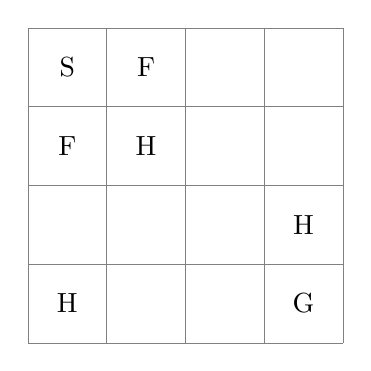
\begin{tikzpicture}[scale=1]
            \draw[step=1cm,gray,very thin] (0,0) grid (4,4);
            \node at (0.5,3.5) {S};
            \node at (3.5,0.5) {G};
            \node at (1.5,2.5) {H};
            \node at (3.5,1.5) {H};
            \node at (0.5,0.5) {H};
            % Add some Fs for detail
            \node at (0.5,2.5) {F};
            \node at (1.5,3.5) {F};
        \end{tikzpicture}
    \end{columns}
    
    \vspace{0.5cm}
    \textbf{Terminal Conditions:}
    \begin{itemize}
        \item Success: Coordinate (3,3) reached.
        \item Failure: Entering any Hole coordinate.
    \end{itemize}
\end{frame}

% 4. Separation of Concerns
\begin{frame}{Separation of Concerns: The Architecture}
    \begin{alertblock}{1. World (Physics Engine)}
        Pure logic. Manages state (x,y), transitions, and valid moves. Knows nothing about language.
    \end{alertblock}

    \begin{exampleblock}{2. Wrapper (Translator Layer)}
        Converts World State $\to$ Text Description.\\
        Parses XML Actions $\to$ World Commands.
    \end{exampleblock}

    \begin{block}{3. Agent (The Brain)}
        Stateless LLM (Gemini). Receives text, outputs XML.
    \end{block}

    \begin{block}{4. Verifier (The Judge)}
        External functions that evaluate the trajectory for correctness and efficiency.
    \end{block}
\end{frame}

% 5. How the LLM Sees the World
\begin{frame}[fragile]{How the LLM Sees the World}
    The Wrapper converts the grid state into a textual prompt context.
    
    \begin{columns}
        \column{0.95\textwidth}
        \begin{lstlisting}[basicstyle=\ttfamily\scriptsize, frame=single, breaklines=true]
You are an RL agent playing FrozenLake 4x4.
Your goal is to reach the Goal (G) from Start (S).

THE MAP LAYOUT (Use coordinates):
- Row 0: S (Start), F, F, F
- Row 1: F, H (Hole!), F, F
...
COORDINATE LOGIC:
- You are currently at (0, 0).
- Goal is at (3, 3).
- DANGER: Do NOT go to (1, 1). That is a HOLE.

Choose the safest path to (3,3).
        \end{lstlisting}
    \end{columns}
    
    \vspace{0.2cm}
    \textit{Note: No numeric tensors. Pure semantic reasoning.}
\end{frame}

% 6. How the LLM Acts
\begin{frame}[fragile]{How the LLM Acts}
    The Agent must output strictly formatted XML.
    
    \begin{block}{LLM Output Example}
        \begin{verbatim}
<thought>
I need to move East to avoid the hole below.
</thought>
<action>RIGHT</action>
        \end{verbatim}
    \end{block}

    \begin{itemize}
        \item \textbf{Why XML?} reliable parsing via Regex.
        \item \textbf{Strictness:} The \texttt{XMLParser} extracts content between tags. 
        \item Invalid format = No Action (or Penalty).
    \end{itemize}
\end{frame}

% 7. Episode Execution Loop
\begin{frame}{Episode Execution Loop}
    The main interactions within \texttt{FrozenLakeEnvironment}:
    
    \begin{enumerate}
        \item \textbf{RESET}: World resets to (0,0). System Prompt prepared.
        \item \textbf{OBSERVE}: Agent receives map info + history.
        \item \textbf{ACT}: Agent generates \texttt{<action>COMMAND</action>}.
        \item \textbf{PARSE}: Wrapper extracts \texttt{COMMAND}.
        \item \textbf{EXECUTE}: World updates state $(x,y) \to (x', y')$.
        \item \textbf{FEEDBACK}: Wrapper generates "You moved to (0,1)...".
        \item \textbf{REPEAT}: Until Goal or Hole reached.
    \end{enumerate}
\end{frame}

% 8. Training vs Evaluation
\begin{frame}{Training vs. Evaluation}
    \begin{columns}
        \column{0.5\textwidth}
        \begin{alertblock}{Gym/RL (Training)}
            \begin{itemize}
                \item Backpropagation
                \item Weight Updates (finding $\theta^*$)
                \item Thousands of episodes
                \item "Learning from params"
            \end{itemize}
        \end{alertblock}
        
        \column{0.5\textwidth}
        \begin{exampleblock}{LLM Agent (Evaluation)}
            \begin{itemize}
                \item \textbf{Frozen Weights} (No backprop)
                \item In-Context Learning
                \item Prompt Engineering
                \item "Learning from History buffer"
            \end{itemize}
        \end{exampleblock}
    \end{columns}
    
    \vspace{0.5cm}
    \centering
    \textit{We are evaluating the model's \textbf{pre-trained reasoning capabilities}, not training it.}
\end{frame}

% 9. Role of Verifiers
\begin{frame}{Role of Verifiers}
    Verifiers are \textbf{external judges} that run after the episode.
    
    \begin{itemize}
        \item \textbf{Success Verifier}:
        Did \texttt{final\_outcome == "goal"}? (Binary)
        
        \item \textbf{Fatality Verifier}:
        Did \texttt{final\_outcome == "hole"}? (Binary)
        
        \item \textbf{Efficiency Verifier}:
        $$ Score = \frac{1}{\text{steps} + 1} $$
        (Higher score for optimal paths).
        
        \item \textbf{Format Verifier}:
        Did the model output valid XML tags?
    \end{itemize}
\end{frame}

% 10. Full Architecture Diagram
\begin{frame}{Full Architecture Diagram}
    \centering
    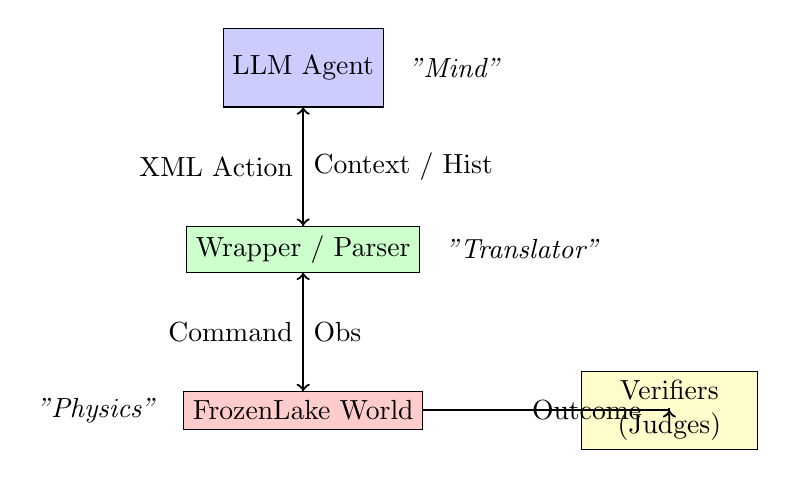
\begin{tikzpicture}[node distance=1.5cm, auto]
        % Nodes
        \node (agent) [rectangle, draw, fill=blue!20, minimum height=1cm, minimum width=2cm] {LLM Agent};
        \node (wrapper) [rectangle, draw, fill=green!20, below=of agent, minimum width=2.5cm] {Wrapper / Parser};
        \node (world) [rectangle, draw, fill=red!20, below=of wrapper, minimum width=2cm] {FrozenLake World};
        \node (verifier) [rectangle, draw, fill=yellow!20, right=2cm of world, text width=2cm, align=center] {Verifiers\\(Judges)};

        % Edges
        \draw[->, thick] (agent) -- node[left] {XML Action} (wrapper);
        \draw[->, thick] (wrapper) -- node[left] {Command} (world);
        \draw[->, thick] (world.east) -| node[pos=0.2, right] {Outcome} (verifier);
        \draw[->, thick] (world) -- node[right] {Obs} (wrapper);
        \draw[->, thick] (wrapper) -- node[right] {Context / Hist} (agent);
        
        % Annotations
        \node [right=0.2cm of agent] {\textit{"Mind"}};
        \node [right=0.2cm of wrapper] {\textit{"Translator"}};
        \node [left=0.2cm of world] {\textit{"Physics"}};
    \end{tikzpicture}
\end{frame}

% 11. Why This Matters
\begin{frame}{Why This Matters}
    \begin{itemize}
        \item \textbf{Reasoning Benchmarks}: Can LLMs plan spatially without visual inputs?
        \item \textbf{Agentic Workflows}: Validates the "Think $\to$ Act $\to$ Observe" loop.
        \item \textbf{Structured Output}: Tests ability to adhere to strict XML protocols under pressure.
        \item \textbf{Memory}: Tests the model's ability to track position history in context window.
    \end{itemize}
\end{frame}

% 12. Final Summary
\begin{frame}{Summary}
    \begin{block}{Key Takeaways}
        \begin{enumerate}
            \item \textbf{World} provides the rules, \textbf{Wrapper} provides the language.
            \item \textbf{Agent} uses In-Context Learning, not gradient descent.
            \item \textbf{Verifiers} ensure rigorous, code-based grading of soft-agent outputs.
        \item The entire system is modular: Swap the LLM, keep the World.
        \end{enumerate}
    \end{block}
    
    \vspace{1cm}
    \centering
    \Large \textbf{Any Questions?}
\end{frame}

\end{document}
